\subsubsection{KP02. Manajemen Transaksi Lelang}
\label{kp02}
	\begin{figure}[H]
		\centering
		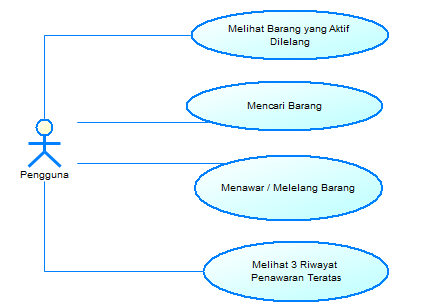
\includegraphics
		[width=\textwidth]
		{images/bab3/usecasediagram/ucd-02.png}
		\caption{Diagram Kasus Penggunaan Manajemen Traksaksi Lelang}
		\label{ucd.02}
	\end{figure}
Pada kasus penggunaan ini, pengguna akan dapat memanajemen transaksi dan penawaran-penawaran yang ia berikan terhadap barang yang terdaftar dalam alikasi.\\


	% Melihat daftar barang yang dilelang
	% Melihat daftar barang yang dilelang

\begin{table}[H]
	\centering
	\caption{Spesifikasi Kasus Penggunaan : Melihat barang yang dilelang}
	\label{uc02.01}
	\begin{tabular}{|r|p{8cm}|}
		\hline
		\textbf{Kode}                                                    & UC-02.01                                                     \\ \hline
		\textbf{Nama}                                                    
			& \textbf{Melihat daftar barang yang dilelang}                                         
			\\ \hline
		\textbf{Aktor}                                                   & Pengguna                                                    \\ \hline
		\textbf{Deskripsi}
			& Pengguna melihat daftar barang yang sedang dilelang
			\\ \hline
		\textbf{Tipe}                                                    
			& Fungsional
			\\ \hline
		\textbf{\textit{Pre Condition}}
			& Sistem belum menampilkan daftar barang yang sedang dilelang
			\\ \hline
		\textbf{\textit{Post Condition}}
			& Sistem menampilkan daftar barang yang sedang dilelang
			\\ \hline
		\multicolumn{2}{|c|}{\textbf{Alur Kejadian Normal}}                                                                            \\ \hline
		\multicolumn{1}{|l|}{}                                           & 
		\begin{enumerate}
			\item Pengguna mengklik \textit{icon} aplikasi di kiri atas halaman
			\item Sistem menampilkan halaman depan yang berisi daftar barang yang sedang dilelang
				  \newline
				  \textit{Ket : Pada halaman depan, ditampilkan barang sesuai dengan kategori berdasarkan waktu dan popularitas, seperti Hot Item (barang yang paling ramai transaksi bidnya), Newest Item, dll.}
		\end{enumerate}
		\\ \hline
		\multicolumn{2}{|c|}{\textbf{Alur Kejadian Alternatif}}                                                         \\ \hline
		\multicolumn{1}{|l|}{}                                           
			& -
		\\ \hline
	\end{tabular}
\end{table}
	
	% Mencari barang yang diinginkan
	% Mencari Barang Lelang

\begin{table}[H]
	\centering
	\begin{tabular}{|r|p{8cm}|}
		\hline
		\textbf{Kode}                                                    
			& UC-02.02                                                     
			\\ \hline
		\textbf{Nama}                                                    
			& \textbf{Mencari Barang Lelang}                                         
			\\ \hline
		\textbf{Aktor}                                                   
			& Pengguna                                                    
			\\ \hline
		\textbf{Deskripsi}
			& Pengguna ingin mencari barang lelang dengan kriteria nama tertentu
			\\ \hline
		\textbf{Tipe}                                                    
			& Fungsional
			\\ \hline
		\textbf{\textit{Pre Condition}}
			& Pengguna menemukan barang lelang yang ia cari dengan kriteria \textit{string}.
			\\ \hline
		\textbf{\textit{Post Condition}}
			& Pengguna menemukan barang lelang yang ia cari dengan kriteria \textit{string} masukan.
			\\ \hline
			\multicolumn{2}{|c|}
			{\textbf{Alur Kejadian Normal}} 
			\\ \hline
		\multicolumn{1}{|l|}{} &
			\begin{enumerate}
				\item Pengguna memasukkan kriteria \textit{string }pencarian di \textit{field} masukan di \textit{Header Bar}
				\item Setelah selesai, pengguna mengklik tombol "Cari"
				\item Sistem mencari barang terdaftar yang sesuai dengan kriteria masukan pengguna
				\item \label{uc0202-a} Jika ketemu, sistem menampilkan halaman "Hasil Pencarian" beserta barang yang sesuai dengan kriteria pengguna.
				\item Pengguna lalu mengklik barang yang sesuai dengan keinginan
				\item Sistem menampilkan detail barang yang sesuai dengan keinginan pengguna
			\end{enumerate}
			\\ \hline
		\multicolumn{2}{|c|}
			{\textbf{Alur Kejadian Alternatif}} 
			\\ \hline
		\multicolumn{1}{|l|}{}                                           
			& \textbf{Tidak ada barang terdaftar dalam sistem yang sesuai dengan kriteria pengguna.}
			\\ \hline
		\multicolumn{1}{|l|}{} & 
			\begin{itemize}
				\item[\ref{uc0202-a}]a. Sistem tidak dapat menemukan barang yang sesuai
				\item[\ref{uc0202-a}]b. Sistem menampilkan "Hasil Pencarian" namun dengan keterangan "Hasil pencarian kosong"
			\end{itemize}
			\\ \hline
	\end{tabular}
	\caption{Spesifikasi Kasus Penggunaan : Mencari Barang Lelang}
	\label{uc02.02}
\end{table}	

	
	% Menawar/melelang barang
		% Menawar/melelang barang
	
	\begin{table}[H]
		\centering
		\caption{Spesifikasi Kasus Penggunaan : Mencari Barang Lelang}
		\label{uc02.03}
		\begin{tabular}{|r|p{8cm}|}
			\hline
			\textbf{Kode}                                                    
			& UC-02.03                                                     
			\\ \hline
			\textbf{Nama}                                                    
			& \textbf{Mencari Barang Lelang}                                         
			\\ \hline
			\textbf{Aktor}                                                   
			& Pengguna                                                    
			\\ \hline
			\textbf{Deskripsi}
			& Pengguna ingin mencari barang lelang dengan kriteria nama tertentu
			\\ \hline
			\textbf{Tipe}                                                    
			& Fungsional
			\\ \hline
			\textbf{\textit{Pre Condition}}
			& Pengguna menemukan barang lelang yang ia cari dengan kriteria \textit{string}.
			\\ \hline
			\textbf{\textit{Post Condition}}
			& Pengguna menemukan barang lelang yang ia cari dengan kriteria \textit{string} masukan.
			\\ \hline
			\multicolumn{2}{|c|}
			{\textbf{Alur Kejadian Normal}}
			\\ \hline
			\multicolumn{1}{|l|}{} & 
			\begin{enumerate}
				\item Pengguna memasukkan kriteria \textit{string }pencarian di \textit{field} masukan di \textit{Header Bar}
				\item Setelah selesai, pengguna mengklik tombol "Cari"
				\item Sistem mencari barang terdaftar yang sesuai dengan kriteria masukan pengguna
				\item \label{uc0202-a} Jika ketemu, sistem menampilkan halaman "Hasil Pencarian" beserta barang yang sesuai dengan kriteria pengguna.
				\item Pengguna lalu mengklik barang yang sesuai dengan keinginan
				\item Sistem menampilkan detail barang yang sesuai dengan keinginan pengguna
			\end{enumerate}
			\\ \hline
			\multicolumn{2}{|c|}
			{\textbf{Alur Kejadian Alternatif}} 
			\\ \hline
			\multicolumn{1}{|l|}{}                                           
			& -
			\\ \hline
		\end{tabular}
	\end{table}	
	
	
	% Melihat 3 riwayat transaksi penawaran harga teratas
	% Melihat Riwayat Penawaran Lelang Barang

\begin{table}[H]
	\centering
	\begin{tabular}{|r|p{8cm}|}
		\hline
		\textbf{Kode}                                                    
		& UC-02.04                                                    
		\\ \hline
		\textbf{Nama}                                                    
		& \textbf{Melihat 3 Riwayat Penawaran Lelang Barang Teratas}                                         
		\\ \hline
		\textbf{Aktor}                                                   
			& Pengguna                                                    
			\\ \hline
		\textbf{Deskripsi}
			& Pengguna ingin melihat riwayat penawaran lelang terhadap barang yang ia daftarkan
			\\ \hline
		\textbf{Tipe}                                                    
			& Fungsional
			\\ \hline
		\textbf{\textit{Pre Condition}}
			& Pengguna menemukan barang lelang yang ia cari dengan kriteria \textit{string}.
			\\ \hline
		\textbf{\textit{Post Condition}}
			& Pengguna menemukan barang lelang yang ia cari dengan kriteria \textit{string} masukan.
			\\ \hline
		\multicolumn{2}{|c|}{\textbf{Alur Kejadian Normal}}
			\\ \hline
		\multicolumn{1}{|l|}{} & 
			\begin{enumerate}
				\item Pengguna membuka halaman "Kelola Barang"
				\item Pengguna mengklik barang yang ingin dilihat informasi riwayat penawaran lelangnya
				\item Sistem menampilkan halaman informasi barang tersebut
				\item Pengguna mengklik tombol "Lihat Penawaran Teratas"
				\item Sistem menampilkan \textit{modal} berisi 3 riwayat penawaran lelang teratas barang tersebut.
				%\item Pengguna memasukkan kriteria \textit{string }pencarian di \textit{field} masukan di \textit{Header Bar}
				%\item \label{uc0202-a} Jika ketemu, sistem menampilkan halaman "Hasil Pencarian" beserta barang yang sesuai dengan kriteria pengguna.
			\end{enumerate}
			\\ \hline
		\multicolumn{2}{|c|}
		{\textbf{Alur Kejadian Alternatif}} 
		\\ \hline
		\multicolumn{1}{|l|}{}                                           
		& -
		\\ \hline
	\end{tabular}
	\caption{Spesifikasi Kasus Penggunaan : Melihat Riwayat Penawaran Lelang Barang}
	\label{uc02.04}
\end{table}	